\documentclass[12pt]{article}
\pdfoutput=1
\usepackage{graphicx,amsmath,amsfonts,amssymb,stmaryrd,latexsym,url,subcaption,hyperref,mathtools,float,cite}
\usepackage[symbol]{footmisc}


\setlength{\textheight}{22.0cm} \setlength{\topmargin}{-1.18cm}
\setlength{\textwidth}{16.0cm} \setlength{\parskip}{0.12cm}
\setlength{\rightmargin}{0.7cm} \hoffset=-1.00 true cm
\addtolength{\abovedisplayskip}{3.0mm}
\addtolength{\belowdisplayskip}{3.0mm}
\addtolength{\abovedisplayshortskip}{3.0mm}
\addtolength{\belowdisplayshortskip}{3.0mm}
%
\addtolength{\footnotesep}{2.0mm}


\begin{document}

\baselineskip=18pt \pagestyle{plain} \setcounter{page}{1}


\begin{center}

{\Large \bf Benefits of marriage as a search strategy} \\ [9mm]



{\normalsize \bf Davi B. Costa\footnote[2]{davicosta@uchicago.edu} \\ [3mm]
{\small \it Physics Department, University of Chicago, Chicago, IL 60637, USA}}

%\center{December 18, 2019}
% \maketitle

\end{center}

\vspace*{0.2cm}


\begin{abstract}
We propose and study an agent-based model of marriage. Agents have preferences that are determined by a probability distribution. They search for better mates through a stochastic matching process, forming new couples and splitting up in the process. Marriage corresponds to the behavior of stopping searching for a better mate when the affinity between a couple exceeds a certain value. We show that the average utility in the system with marriage can be higher than in the system without it. Part of our results can be summarized in what sounds to be good advice: don’t marry the first person you like or search for the love of your life, but get married if you like your partner more than a sigma above average. To test the adequacy of our model to describe real societies, we compare the evolution of the fraction of married couples to real-world data and obtain good agreement.
\end{abstract}



\newpage


\newpage
\section{Introduction}

Consider the following situation: you are wondering whether to propose marriage to your partner. There are many aspects of marriage to consider, but you are mainly concerned with marriage as a ``search strategy". You like your partner, but aren't sure if it's enough. After all, there may be someone else out there who you prefer even more, but you are unlikely to meet this person if you marry. Perhaps, from a ``search strategy" perspective,  the best option is to avoid marriage and remain open to the chance of meeting a better match. However, if your relationship is symmetrical in this regard, you may find yourself single because your partner has moved on. As a result, while marriage reduces some of the opportunities that would otherwise be available to you, it also protects you from being left out. So you ask yourself: is getting married a good search strategy? In other words, does the possibility of meeting someone with whom you have a higher affinity outweigh the risk of being alone because your current partner has left you?

A famous problem related to this subject is the stable matching problem \cite{10.2307/2312726}. It is the problem of finding a stable matching between two groups of agents with preferences among themselves. If we interpret the groups as man and woman, then a matching is a bijection between these two genders, and a matching is stable if there are no man and woman who both prefer each other over their respective mate. Since its inception, there has been extensive research on the mathematical structure of stable matching and related algorithmic questions \cite{10.2307/2312726,knuthstable,gusfield1989stable,roth1992two}. The notion of stable matching is fundamental to understand a variety of markets, as one can find in the recent review \cite{ren2021matching}. Furthermore, matching theory is a relevant tool for market design \cite{article,NBERw29367}. However, when it comes to large societies, the concept of stable matching may not be important. After all, it is likely that there are two agents that would rather be together than be with their respective mates. But, in a large society, this blocking pair may not yet know each other. Also, the likelihood that this will happen depends on the type of relationship they have. If they are married, in principle, they will not be open to this possibility. Otherwise, they may eventually match a better mate. To make these ideas precise and to answer the question from the previous paragraph, we propose a agent-based model of marriage based on a random matching process and simple behavioral rules.

The model contains a number $N$ of agents with preferences among themselves sampled by a Gaussian distribution. Initially, all agents are singles, and the system evolves in a certain number $T$ of discrete steps. At each step, they will match in pairs by random chance. If the agents of the matched pair like each other more than their previous mates, or more than being single, they will form a new couple. An agent becomes single if its partner starts a new relationship. Marriage is modeled by adding the behavior of stopping searching for a better mate when two agents like each other by more than a certain individual cutoff parameter. We assumed the set of cutoff parameters is also normally distributed and we simulate the system for different values for the average of this distribution. In each case, we computed the average utility as a function of the number of steps. Part of the conclusions one can extract from the results we obtained answers the question from the first paragraph. The answer can be summarized in what sounds to be good advice: \textit{don’t marry the first person you like or search for the love of your life, but get married if you like your partner more than a sigma above average}. In addition, the output of the simulation allows one to test the adequacy of the model to describe real societies: one can compare the fraction of married couples at each step in our model with the fraction of persons of a given generation that are married at a certain age for real societies. This was done by comparing Fig. (\ref{mcsimulation}) and Fig. (\ref{mcrealdata}), which arguably gives a good agreement when taken into account the purposeful simplicity of our model.


%Our approach differ in a number of ways from other search models. In our model, search frictions are associated with the possibility of being left. In addition, we did not concentrate on the steady state. (For a detailed presentation see, for instance, Pissarides 1990, Shimer & Smith 2000, Smith 2011.). The fraction of married couples, unmarried couples and singles, changes as our model evolves. Interpreted, moreorless as a generation, this dynamics gives one of the empirical avenues to test the model.

%Becker (1973,1974) was the first to point out that the tools of economic analysis could be applied to the analysis of such demographic phenomena as marriage.

The idea of using formal tools for the study of marriage is not new \cite{10.2307/1831130,10.2307/1829987,10.2307/1837421}. Following the recent taxonomy for models of the marriage market proposed in \cite{doi:10.1146/annurev-economics-012320-121610}, our model fits best in the category of search models (see \cite{10.2307/23045893,10.1257/002205105775362014,doi:10.1146/annurev-economics-111809-125046,10.1257/jel.20150777} for a detailed presentation of the work in search theory, and  \cite{10.2307/2780247,10.2307/2951279,Burdett1999LongTermPF,10.2307/2999430,10.2307/44955185,RePEc:bpj:bejmac:v:advances.1:y:2001:i:1:n:5} for examples of search models of marriage). However, our approach is different from these works. Instead of analysing matching properties for generic preferences, as most referenced works have done, we assumed a probability distribution for the preferences and proposed a specific matching process. The motivation for adopting a probability distribution stems from our interest in the limit $N\gg T$, i.e., when the number of agents is substantially more than the number of times agents match one another. When compared to other works that do not assume completely generic preferences \cite{doi:10.1086/689869,10.1093/restud/rdw041}, we give less structure to agents' preferences in this way. Besides, our proposed matching process was an attempt to model how people match in real societies. Thus, our model is similar in approach to some works in complexity economics \cite{comecon,10.5555/547051}, and it illustrates a case where one of conventional economics' assumptions does not hold. To be concrete, the dynamics of our model are driven by simple behavioral rules. However, the overall pattern of evolution is complex and no agent have the computational power to calculate which behavior will lead to maximum average utility. As a result, utility maximization does not appear to be dictating the behavior of agents in these scenarios.


\section{The mate-search model}
\label{dynamicalmatching}

The mate search model is the backbone of the marriage model we are going to present in the next section. It contains $N$ agents with preferences among themselves described by a utility function \cite{mas1995microeconomic}. This information is encoded in the off-diagonal elements of the \textit{affinity matrix} $A\in\mathbb{R}^{N\times N}$, where $A_{ij}$ is the utility for agent $i$ to be in a couple with agent $j$. Note that $A$ is not symmetric in general because the utility for agent $i$ to be with agent $j$ is not necessarily the same as the reverse. In addition, $A_{ij}$ is not positive in general, as it's common to find people you'd rather be single than date. %The diagonal entries of the affinity matrix are interpreted as the utilities when the agents are singles. 
We will often refer to the collection of agents of our model as the society.

In large societies, the probability distribution that generates the affinity matrix is more important than its actual values. Indeed, the preferences of agent $k$ concerning the other agents of society are encoded by $\{A_{kj}:1\leq j\leq N\textrm{ and } j\neq k\}$, which is distributed according to some probability distribution. As it happens with many human traits, it may be reasonable to assume that these values are distributed normally, i.e., $A_{kj}\sim\mathcal{N}(\mu_k,\sigma_k)$ for all $1\leq j\leq N$ with $j\neq k$ and each $1\leq k\leq N$. In principle, one may think that it is more realistic to assume that the preferences of different agents are given by distributions defined with different parameters $\mu$ and $\sigma$. Note, however, that the values of the $k-$column of the affinity matrix, $\{A_{jk}:1\leq j\leq N\textrm{ and } j\neq k\}$, encodes the way agent $k$ is liked by society. Therefore, if agents indeed have preferences given by different Gaussian distributions, then the distribution that generates the columns of the affinity matrix will not in general be Gaussian. Hence, to have both lines and columns consistently Gaussian, we may assume that all off-diagonal entries of the affinity matrix are generated by the same Gaussian distribution, that is $A_{kj}\sim\mathcal{N}(\mu,\sigma)$ for all $1\leq j\leq N$ and $1\leq k\leq N$ with $j\neq k$. When this is the case, we will say that we are dealing with the \textit{Gaussian model}. For comparison, we will also study the \textit{Uniform model}, i.e., $A_{ij}\sim U(\mu-2\sigma,\mu+2\sigma)$. 

The diagonal elements of the affinity matrix are the utilities when agents are singles. We also believe it is reasonable to assume these values are generated by a Gaussian distribution. Note, that the mean of the diagonal elements gives the average utility when all agents are single. On the other hand, the mean of the off-diagonal elements can be interpreted as the average utility when agents form random pairs. Therefore, the relationship between the mean of these two distributions encodes how being single compares to dating a random agent in society. We do not believe this two quantities are generically the same. But, for concreteness, we will present our results assuming they are. However, we will show in section (\ref{discussionandcomments}) that our conclusions still hold when this is not the case.

The dynamics of the system happen in discrete steps $t\in\mathbb{N}$. At each step $t$, all agents match at random with a new agent. More precisely, at each step, there is a random matching between all agents. That is, a bijection

\begin{align}
    \mu_t:\{1,2,\dots,N\} & \rightarrow \{1,2,\dots,N\}
    \label{matching}
\end{align}

\noindent generated by a random process with uniform distribution. The matching $\mu_t$ maps $k$ to $\mu_t(k)$, the agent $k$ match at $t$. Suppose first, that agent $k$ is single at $t$ having $u_t^k=A_{kk}$, and match with agent $l=\mu_{t+1}(k)$ at $t+1$. These two agents will form a couple if they like themselves, more precisely we will have

\begin{align}
    u_{t+1}^k=\begin{cases} A_{kl}, & A_{kl}>u_t^k=A_{kk}\ \textrm{and }\ A_{lk}>u_{t}^l,\\
    u_t^k, & \textrm{otherwise}.
    \end{cases}
    \label{singleevolution}
\end{align}

\noindent Now, suppose agent $k$ is in a couple with agent $m$ at $t$. In this case $u_t^k=A_{km}$ and $u_t^m=A_{mk}$. At step $t+1$, let agent $k$ match with agent $l=\mu_{t+1}(k)$ and $m$ with agent $n=\mu_{t+1}(m)$. Then, if the affinity among matched agents is larger then the affinity between the mates, a new couple will be formed and the old couples will break apart. More precisely

\begin{align}
    u_{t+1}^k=\begin{cases} A_{kl}, & \textrm{if}\quad A_{kl}>u_t^k\ \textrm{and }\ A_{lk}>u_{t}^l,\\
    A_{kk}, & \textrm{if}\quad A_{mn}>u_t^m\ \textrm{and }\ A_{nm}>u_t^n,\\
    u_t^k, & \textrm{otherwise}.
    \end{cases}
    \label{coupleevolution}
\end{align}

\noindent We start the system with all agents as singles, that is $u_0^k=A_{kk}$ for all $1\leq k\leq N$. We should emphasize that here, a couple is not a married couple. We will introduce marriage in the next section. 

Running the simulation by $T$ steps produces a $N\times T$ matrix $\{u_t^k:1\leq k\leq N,1\leq t\leq T\}$ that gives the utility of agent $k$ at each step $t$. As we are interested in large societies $T\ll N$, we are more interested in the average utility and its variance:

\begin{align}
    u_t\equiv\frac{1}{N}\sum_{k=1}^Nu_t^k,\qquad \sigma_t\equiv\frac{1}{N}\sqrt{\sum_{k=1}^N(u_t^k)^2-\Big(\sum_{k=1}^Nu_t^k\Big)^2}
\end{align}

\noindent (in fact, all moments carry aggregate information of the system, but we will postpone its systematic study to future work). The marked difference between $u_t^k$ and $u_t$ can be visualized by plotting their values for a simulation of the Gaussian $\mathcal{N}(0,1)$ model with $N=10.000$:


\begin{figure}[H]
\begin{subfigure}{.49\textwidth}
  \centering
  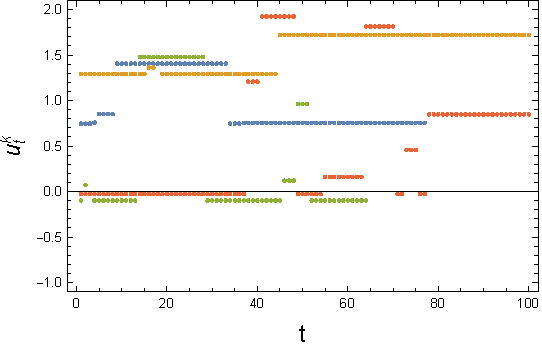
\includegraphics[width=\linewidth]{uktGn10000s1l1.pdf}
\end{subfigure}%
\begin{subfigure}{.49\textwidth}
  \centering
  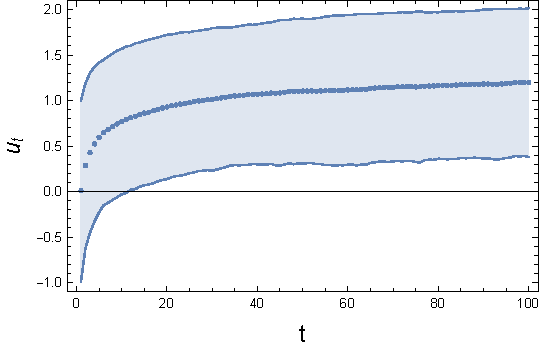
\includegraphics[width=\linewidth]{utGn10000s1l1.pdf}
\end{subfigure}
\caption{Evolution of the utility of four agents distinguished by color (left) and average utility with band equal to the variance  (right). In both cases we have the Gaussian model $\mathcal{N}(0,1)$ with $N=10.000$.}
\label{ukut}
\end{figure}

\noindent The plot for the Uniform model $U(-2,2)$, which has variance $\sigma=1$, is very similar and hardly distinguishable visually from the above ones.

As in Fig. (\ref{ukut}), the results we will present were obtained in simulations using $\mu=0$ and $\sigma=1$. However, for the case that all entries of the affinity matrix are given by the same distribution, there is a symmetry that allow us to translate the results to generic $\mu$ and $\sigma$. Note, that the dynamical equations (\ref{singleevolution}) and (\ref{coupleevolution}), depends on inequalities between values of the affinity matrix such as $A_{ij}>A_{kl}$. This fact implies that the dynamics of the system will be the same if we shift and re-scale all values of the affinity matrix $A_{ij}\rightarrow\tilde{A}_{ij}=\sigma A_{ij}+\mu$. But this corresponds to using generic $\mu$ and $\sigma$ instead of 0 and 1. By doing so, the utility of each agent at each step will shift and re-scale accordingly, that is $u_t^k\rightarrow \sigma u_t^k+\mu$. Hence we can translate the results obtained for $\mu=0$ and $\sigma=1$ to generic $\mu$ and $\sigma$. In symbols, we have:

\begin{align}
    \textrm{if}\qquad(\mu=0,\sigma=1)\mapsto u_t^k\qquad\textrm{then}\qquad (\mu,\sigma)\mapsto \sigma u_t^k+\mu.
    \label{generalmusigma}
\end{align}

\noindent Using this dictionary we can easily translate the results of Fig. (\ref{ukut}) to general $\mu$ and $\sigma$. We will have $u_t^k\rightarrow \sigma u_t^k+\mu$ and $u_t\rightarrow \sigma u_t+\mu$. Therefore, it suffices to think of $0$ as $\mu$ and interpret the units of the vertical axis as given in terms of $\sigma$.


As stressed before, in large societies the number of matchings we have during our lifetimes is much smaller than the number of agents that make our societies $T\ll N$. In particular, the asymptotic limit $T\rightarrow\infty$ doesn't seem to be important. This resonates with the famous Keynes quote ``in the long run we are all dead" \cite{keynes1923tract}, which can be read as the advice that asymptotic limits and equilibrium states are not always relevant. In addition, the asymptotic limit $T\rightarrow\infty$ does not approach any equilibrium state in this model. Imagine for simplicity 3 agents, $A,B$ and $C$. Suppose $A$ has higher affinity with agent $C$, $B$ with $C$, and $C$ with $A$. At each step one of the agents does not match and they will remain in an eternal dance, which is not uncommon in modern relationships. The fact that this system never stabilizes shows that even generalized concepts of stability \cite{Multi-period,doval2021dynamically,Credibility,DAMIANO200534} may not be important to understand the matching of couples in large societies.


\section{The marriage model and results}
\label{benefitsofmarriage}

The marriage model is an extension of the mate search model by the following additions. First, we introduce the \textit{proposal vector} $\vec{\Lambda}\in\mathbb{R}^N$, where $\Lambda_k$ encodes how much agent $k$ needs to like another agent to propose marriage. Then, if the affinity between a couple is higher than their respective proposal values, the couple will not match with new agents in the next steps of the evolution. In this case, we say that the couple is married. More precisely, 

\begin{align}
    \textrm{the $(k,l)$-couple is married at $t$ if}\qquad u^k_t=A_{kl}>\Lambda_k\qquad \textrm{and}\qquad u^l_t=A_{lk}>\Lambda_l.
    \label{marriedcoupled}
\end{align}

\noindent Let $\mathcal{M}_{t}\subseteq\{1,2,\dots N\}$ be the set of agents married at time $t$, then the matching at time $t+1$ will not include them

\begin{align}
    \mu_{t+1}^\Lambda:\{1,2,\dots,N\}-\mathcal{M}_{t}\rightarrow\{1,2,\dots,N\}-\mathcal{M}_{t},
    \label{marriedcouples}
\end{align}

\noindent where $\{1,2,\dots,N\}-\mathcal{M}_{t}=\mathcal{M}^c_t$ is the complement of $\mathcal{M}_t$ over $\{1,2,\dots,N\}$, that is, the set of unmarried agents at time $t$.

As we argued before, for a large society, what is important is the distribution that samples the values of the proposal vector $\vec{\Lambda}$ and a reasonable assumption is that $\Lambda_k\sim\mathcal{N}(\Lambda,\sigma_\Lambda)$. One can think of the values $\Lambda$ and $\sigma_\Lambda$ as exogenous in the sense that they characterizes the behavior of the agents of a given society. Different societies (or the same society in different moments of time) will have different values of $\Lambda$. This will become clear with the discussion following the comparison between Fig. (\ref{mcsimulation}) and Fig. (\ref{mcrealdata}) in the next section. In what follows, to facilitate the investigation of the model, we will further take the limit $\sigma_\Lambda\rightarrow0$, so that $\Lambda_k=\Lambda$ for all $1\leq k\leq N$.

As in Eq. (\ref{generalmusigma}), results obtained using $\mu=0$, $\sigma=1$ can be translated to results obtained for generic $\mu$ and $\sigma$. However, from Eq. (\ref{marriedcoupled}) with $\Lambda_k=\Lambda_l=\Lambda$, one sees that it is necessary to shift and re-scale $\Lambda$ to preserve the dynamic. More precisely, let $u_t^k$ be the utility of agent $k$ obtained for $\mu=0$, $\sigma=1$ and $\Lambda$. Then, the simulation for generic $\mu$ and $\sigma$, will give $\sigma u_t^k+\mu$ if one uses $\sigma\Lambda+\mu$ instead of $\Lambda$. In symbols we have:

\begin{align}
    \textrm{if}\qquad (\mu=0,\sigma=1,\Lambda)\mapsto u_t^k\qquad\textrm{then}\qquad (\mu,\sigma,\sigma\Lambda+\mu)\mapsto \sigma u_t^k+\mu.
    \label{dictionarymarried}
\end{align}

\noindent We see that our results are still generic for $\mu$ and $\sigma$ with the appropriate transformation of $\Lambda$.

We can compare the average utility in the system with and without marriage for different values of $\Lambda$. Our results are presented in Fig. (\ref{lcompUG10000s1}) and Fig. (\ref{lcompUN10000s1}). The most significant lessons from our stochastic model can be extracted from these figures. Note that if we have $\Lambda>A_{ij}$ for all $i,j$, then marriage will not affect the dynamics of the system. Therefore, for sufficiently large $\Lambda$ (and finite $N$), the marriage model is equal the mate search model. On the other hand, if $\Lambda<A_{ij}$ for all $i,j$, then every agent will marry with the first matched agent they like, and the average utility will get smaller as one can see from the plots. The lesson we can extract from this result is that we should not get married to the first person we like. However, for some intermediary values of $\Lambda\simeq\sigma$, the average utility is consistently larger in the system with marriage. Therefore, it is reasonable to conclude that we should marry if we like our partner more than a sigma above average. For $\Lambda\simeq\sigma$, the lines cross, therefore, there will be a different value $\Lambda_t$ that maximizes the average utility at different steps $t$. 

\begin{figure}
\centering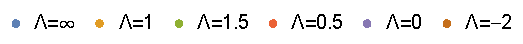
\includegraphics{legend.pdf}
\begin{subfigure}{.49\textwidth}
  \centering
  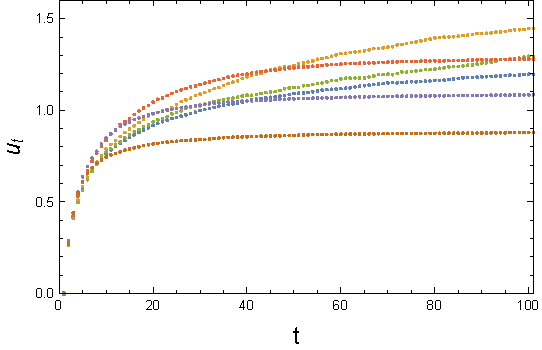
\includegraphics[width=\linewidth]{GLcompN10000s1.pdf}
  \caption{Gaussian model $\mathcal{N}(0,1)$.}
  \label{lcompUG10000s1}
\end{subfigure}%
\begin{subfigure}{.49\textwidth}
  \centering
  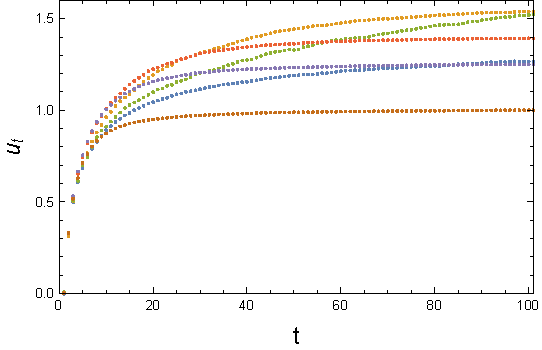
\includegraphics[width=\linewidth]{NewlcompUN10000s1.pdf}
  \caption{Uniform model $U(-2,2)$.}
  \label{lcompUN10000s1}
\end{subfigure}
\caption{Average utility evolution in the Gaussian and Uniform model with $N=10.000$ for different values of $\Lambda$. We used $\Lambda=\infty$ to denote the system without marriage.}
\label{lcomp}
\end{figure}

To help further clarify the possible interpretations of the results, consider the following scenario. During our lives, we can take all opportunities we have to match others, pursuing the dream of finding the greatest love of our lives. Alternatively, after finding someone who makes us happy more than a certain amount, we can decide to stop this search. From the results of this model we may conclude that, on average, it is better to stick with someone good enough than always be looking for the big love of our lives. The conjunction of these results justifies the sentence we advertised before: don't marry the first person you like and don't search for the love of your life, but get married if you like your partner more than a sigma above average.

There is a second interpretation for these results that personally motivated this model. Suppose you are dating, and you should decide if you will engage in monogamy or non-monogamy. The most salient difference is that in non-monogamy, you and your mate would be open to match with others. To decide, you need to consider several features of your preferences. For example, how much you like to match new people periodically. Whether you have enough time to spend with your mate and sporadic matches. How jealous you feel when your mate match with others. To mention but a few. In addition, the openness characteristic of non-monogamous relations increases the chances of matching with someone either you or your mate have more affinity. Hence, you may wonder if the odds of finding someone better pays the cons of being left out by your mate. If one interprets what we called a couple as non-monogamy, and what we called a married couple as monogamy, then the model proposed addresses this question and gives a negative answer. The significant conclusion is that, if you are in all respects unsure whether you prefer monogamy or non-monogamy, the benefit of marriage as a search strategy disclosed by this model should tip the balance in favor of monogamy. Perhaps, in the future, this interpretation will be more significant as the number of people that experience non-monogamous relationships is growing \cite{doi:10.1080/0092623X.2016.1178675}. However, throughout the paper, we will stick to the first interpretation.

It is also interesting to plot the evolution of $u_t$ with the variance as we did in the previous section for the model with and without marriage. In Fig. (\ref{averageutilityandvariance}), we see that the system with marriage and $\Lambda=\sigma$, have a higher mean and a lower variance. If agents value equality with respect to relationships, this fact can be interpreted as another benefit of marriage. 
%At each step, it is possible to count the number of couples in the model. This number divided by $\frac{N}{2}$ ranges between $0$ and $1$ and gives the share of couples in the model at step $t$. We can compare the result for different values of $\Lambda$. Fig. (\ref{sharecouples}) with the share of couples, either married or unmarried, at each step reveals what might be taken by some as another benefit of marriage: the share of couples in the population is larger for a society with marriage.

\begin{figure}
\begin{subfigure}{.49\textwidth}
  \centering
  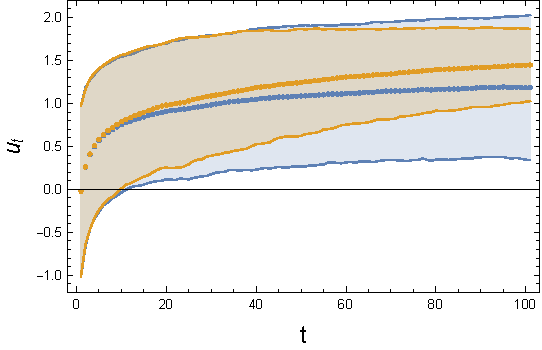
\includegraphics[width=\linewidth]{NewutumtGN10000s1l1.pdf}
  \caption{Gaussian model $\mathcal{N}(0,1)$}
  \label{utumtGn10000s1l1}
\end{subfigure}%
\begin{subfigure}{.49\textwidth}
  \centering
  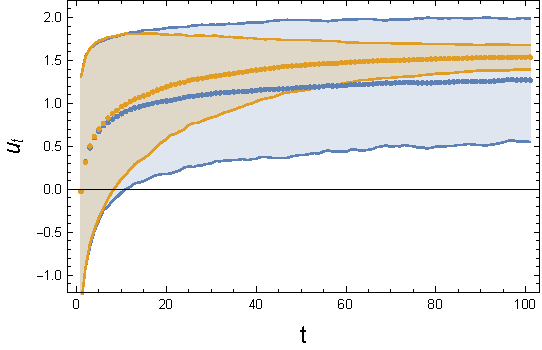
\includegraphics[width=\linewidth]{NewutumtUN10000s1l1.pdf}
  \caption{Uniform model $U(-2,2)$}
  \label{utumtUN10000s1l1}
\end{subfigure}
\caption{Average utility evolution in the the system with marriage and $\Lambda=1$ (orange) and without marriage (blue) in the Gaussian and Uniform models with $N=10.000$.}
\label{averageutilityandvariance}
\end{figure}

It is important to emphasize that the benefits of marriage as a search strategy disclosed using this model may be irrelevant when other aspects of marriage are considered. There are many layers of our preferences concerning relationships that are not taken into account by this model. For example, although an agent that does not marry will end up on average with someone with a lower affinity, it nevertheless may be the case that this agent gets a surplus of utility associated with the fact of participating in multiple relations during his lifetime. As another example, in general it is painful to break apart. However, this loss is not considered in the model. But would rather add another benefit to the society with marriage. Overall, evidence seems to suggest that marriage is beneficial in a number of respects \cite{doi:10.2307/2061670}.

A salient simplification of our model is that in real life, the affinity between agents is not time-independent. It is worth to mention, that if we include a time-dependent affinity, then our model will already include divorce. Indeed, given a married couple, their affinity may get smaller than $\Lambda$. When this happens, the married couple will unmarry and may break apart if one of the participants finds another mate. A time-dependent affinity would also account for the spontaneous break-up of couples. It suffices that the affinity between the couple gets smaller than the utility for one of the mates to be single. Understanding the average dynamical behavior of the affinity between agents is beyond the scope of this paper. %Perhaps, the affinity is an oscillatory function with higher amplitude as the time with a given mate passes. As it often happens, old couples frequently oscillate between high-affinity and low-affinity states.


\section{Discussion, comments and empirical comparison}
\label{discussionandcomments}

A possible point of concern, is the fact that we did not distinguished man and woman as in the original marriage problem \cite{10.2307/2312726}. One could then think that we are actually dealing with something related to the roommate problem instead \cite{10.2307/2312726}. This distinctions, however, are not important for our model. We can partition society into two, making matching just between agents not of the same group. The evolution of average utility for such a system is visually indistinguishable from Fig. (\ref{utumtGn10000s1l1}) and Fig. (\ref{utumtUN10000s1l1}), giving the same pattern and disclosing the same benefits outlined before. One can even partition society into groups of different sizes, and the results are still very similar. For this situation, the matching in Eq. (\ref{matching}) is a random surjective function from the smallest partition to the largest one. A random subset of agents that make the large partition is left out from the matching process at each step. Several variations are possible in this setup. For example, we could select a subset of one of the partitions and make it match with itself as well. This subset could then be interpreted as bisexual agents. This flexibility of our model goes in line with the present diversity of modern relationships and contrasts with results for the matching problem. Many results, such as the Gale-Shapley algorithm, depend on the fact that both sets in the matching process have the same number of elements \cite{roth1992two}.

It is interesting to compare the value for the average utility attained in our model with the value obtained using the Gale–Shapley algorithmic solution to the matching problem \cite{10.2307/2312726}. We use the Gale-Shapley algorithm to find a stable matching and then we computed the average utility associated with it $u_{G-S}$. We did this for different values of $N$. For all $N$ studied, $u_{G-S}$ is much higher than the values obtained in our model. For example, in the Gaussian model with $N\simeq 1.000$ we found $u_{G-S}\simeq 4$. This is another indication that the concept of stable matching is not relevant to understand the matching of couples in large societies. However, the fact that $u_{G-S}$ is larger than $u_t$ for $t\simeq100$, implies that the market of relationships in large societies is sub-optimal. If in the future we are able to infer the affinity between agents using correlated manifest properties, such as age, personality, political bias, level of education, etc., then we could use the Gale-Shapley algorithm to spell a stable matching, and society average utility with respect to relationships would be much higher. 

In addition to Gale-Shapley, one could be interested in a comparison with Becker's paradigm of transferable utility \cite{10.2307/1831130,10.2307/1829987}. In this case, one should try to find the matching $\mu^*:\{1,2,\dots,N\}\rightarrow\{1,2,\dots,N\}$ that maximizes

\begin{align}
    u(\mu)=\frac{1}{2}\sum_{i=1}^N(A_{i\mu(i)}+A_{\mu(i)i}).
\end{align}

\noindent Such matching $\mu^*$ is not necessarily stable, but the average utility is, by definition, maximized in this case. Note, however, that there is a total of $N!$ matchings, which for $N\simeq1.000$ is a $2.568$ digits number. So for large societies, it will be computationally impossible to find $\mu^*$.

As mentioned in section (\ref{dynamicalmatching}), we assumed for concreteness that the diagonal and off-diagonal elements of the affinity matrix are given by the same distribution. So, one might rightly worry that our results are not valid if this is not the case. To address this concern, we simulate our model assuming that $A_{kk}=0$ for all $1\leq k\leq N$ and that $A_{ij}=\mathcal{N}(\mu,1)$ for all $1\leq i\leq N$ and $1\leq j\leq N$ with $i\neq j$, for different values of $\mu$ and $\Lambda=\mu+\sigma=\mu+1$. Note that $A_{kk}=0$ is obtained formally using $\mu=0$ and taking the limit $\sigma\rightarrow0$ for the distribution $\mathcal{N}(\mu,\sigma)$ that generates the diagonal elements of the affinity matrix. Furthermore, in this limit, there is no loss of generality in assuming that $\sigma=1$ for the off-diagonal elements. This happens because, when $A_{kk}=0$ for all $1\leq k\leq N$, the dynamical equations (\ref{singleevolution}) and (\ref{coupleevolution}), are still invariant under re-scaling of $A_{ij}$ and therefore the results obtained for $\sigma=1$ can be translated to generic $\sigma$ as we did in (\ref{generalmusigma}). The simulations shows that there is a ``average utility gap" between the system with marriage and without marriage that grows for large and closes for small values of $\mu$. More precisely, let $f(\mu)\equiv u_{M}(\mu)-u(\mu)$, with $u_M(\mu)$ and $u(\mu)$, respectively, the average utility in the system with marriage ($\Lambda=1$) and without marriage ($\Lambda\gg1$). Then $f(\mu)$ is a monotonically non-decreasing function and $f(\mu)>0$. So the benefit of marriage outlined in the previous section seems to be a robust feature of the model.

Another objection to the results presented in the previous section is that the assumption of a homogeneous society is clearly false. What is interesting, however, is that for a finite number of agents, this homogeneity is already broken. More precisely, for all agents $k$, its affinity with the other agents is given by $\{A_{jk}:1\leq j\leq N\textrm{ and } j\neq k\}$, which is generated by the same distribution but is, in general, a different collection of numbers for each agent in an actual simulation. To make this point more clear consider the following. We can select all agents $k$ such that the average of the collection $\{A_{jk}:1\leq j\leq N\textrm{ and } j\neq k\}$ is larger than a certain positive value. We can pick this value in a way that we have just $1\%$ of all agents selected. This will represent the $1\%$ most liked agents of the system. Conversely, we can do the same and get the $1\%$ less liked agents. It is then interesting to follow the evolution of average utility for these different sets of agents. One finds that marriage is more beneficial to those that are not that liked. This agrees with intuition. If everyone likes you, you should not be concerned with marriage as a search strategy. It is easier for you to find a nice partner that also likes you and your mate is less likely to leave you because of someone else.

It is hard to measure the average utility in a real societies, but the number of married couples is not. By comparing the share of married couples in our model and existent societies we can test the adequacy of our model to describe reality. We have

\begin{figure}[H]
    \centering
    \begin{minipage}{0.47\textwidth}
        \centering
        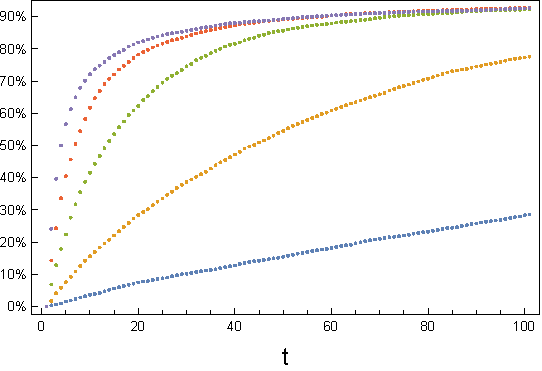
\includegraphics[width=\textwidth]{mclcompUN10000s1.pdf}
        \caption{Share of married agents in the Gaussian model $\mathcal{N}(0,1)$ with $N=10.000$ at each step for different values of $\Lambda$. From the bottom to the upper lines we have $\Lambda=1.5,1,0.5,0,-2$.}
        \label{mcsimulation}
    \end{minipage}\hfill
    \begin{minipage}{0.47\textwidth}
        \centering
        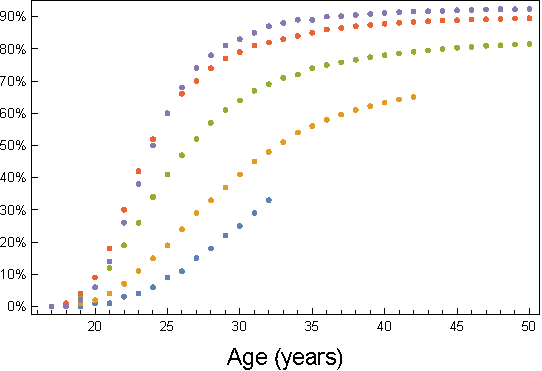
\includegraphics[width=\textwidth]{mcrealdata.pdf}
        \caption{Share of men in England and Wales who were married by a certain age \cite{owidmarriagesanddivorces}. From the bottom to the upper lines we have men who were born at $1980,1970,1960,1950,1940$ respectively.}
        \label{mcrealdata}
    \end{minipage}
\end{figure}

\noindent which is arguably a good agreement when taken into account that we purposely ignore some relevant aspects of marriage, such as divorce. We highlight, though, that we could implement divorce by having a time-dependent affinity, as mentioned in the last paragraph of section (\ref{benefitsofmarriage}). We also call attention to the fact that the similar behavior of the two plots was not built-in our stochastic matching model in any way. It is a pure dynamical consequence. A

The trends of a declining number of married men in Fig. (\ref{mcrealdata}) can be interpreted in the framework of our model as a shift to higher $\Lambda$. This agrees with rough expectations. In the past, marriage was enforced by tradition and many couples get married without high affinity. Progressive movements diminished the forces of tradition and people became more rigorous to get married. If we go further and assume that each generation in Fig. (\ref{mcrealdata}) is associated with a value of $\Lambda$ with the same color in Fig. (\ref{mcsimulation}), we can see in Fig. (\ref{lcompUG10000s1}) that the average utility concerning relationships increased from 1940 to 1970, and perhaps starts decreasing from 1970 to 1980. This being true, would suggest that the progressive movements benefited the matching markets of traditional societies by increasing $\Lambda$. But perhaps, $\Lambda$ went too high and needs to be balanced. The right balance can be achieved following the piece of advice extracted from the results of the previous section: get married if you like your partner more than a sigma above average. As mentioned before, the steps $t$ are likely not linearly related to chronological time. If initial steps are compressed, as it is reasonable to assume, the initial convex behavior of the real-world data in Fig. (\ref{mcrealdata}) may be attained. Most significantly, if approximately correct, this model gives an avenue to access an unobservable quality of society, average utility, using an observable one, the evolution of the fraction of married people.

\section{Conclusions}

We proposed and studied an agent-based model of mate searching and marriage in large societies based on a stochastic matching process and simple behavioral rules. By investigating this model, we disclosed some benefits of marriage as a search strategy. Most significantly, the average utility in the system with marriage can be higher than in the system without it. We summarized some of our results in what sound to be good advice: don't marry the first person you like and don't search for the love of your life, but get married if you like your partner more than a sigma above average. We also mentioned that the average utility attained in our stochastic model is smaller than the one associated with a stable matching achieved using the Gale-Shapley algorithm. This can be taken as a simulation-based argument in favor of a central planner (perhaps an app) with the information to coordinate the marriage market in order to set a stable matching. To roughly test the adequacy of our model to describe real societies, we compared the evolution of the fraction of married couples to real-world data and obtained good agreement.

This work left open many directions for investigation. For those interested in the adequacy of this model to describe reality, it would be important to do a more systematic comparison between the fraction of couples in our model and real societies, as we did in Fig. (\ref{mcsimulation}) and Fig. (\ref{mcrealdata}). One could try to model a mapping between steps of evolution and chronological time. By doing so, it would be easier to infer $\Lambda$ from the fraction of couples and one would be able to discover the value of $\Lambda$ for different societies. Combined with our study of the average utility as a function of $\Lambda$, summarized in Fig. (\ref{lcomp}), one could then advise the agents of a given society to be more or less selective to get married. For those interested in extending the model, it would be relevant to investigate the fact that the affinity of a couple changes as time together passes. With a dynamical affinity, it would be possible to investigate new connections with real data, as the rate of divorce. Furthermore, it would be nice to use more formal tools to demonstrate in a more analytic form the lessons from the model. As we have just shown, there are many open directions to advance the understanding of our stochastic matching model. Hopefully, this study will pave the way for future works.


\vspace{5mm}
\noindent
\textit{Acknowledgments:} This work was motivated by personal experiences with my girlfriend Lis, whom I thank for her love and companionship. As I am sure that our affinities are more than one sigma above the average, I hope the results presented here will convince her that we should get married, as they have convinced me.

\newpage
\bibliographystyle{unsrt}
\bibliography{bib}


\end{document}